


\chapter*{Implementation - Architecture}
\addcontentsline{toc}{chapter}{Architecture}


  \begin{figure}
    \begin{center}
      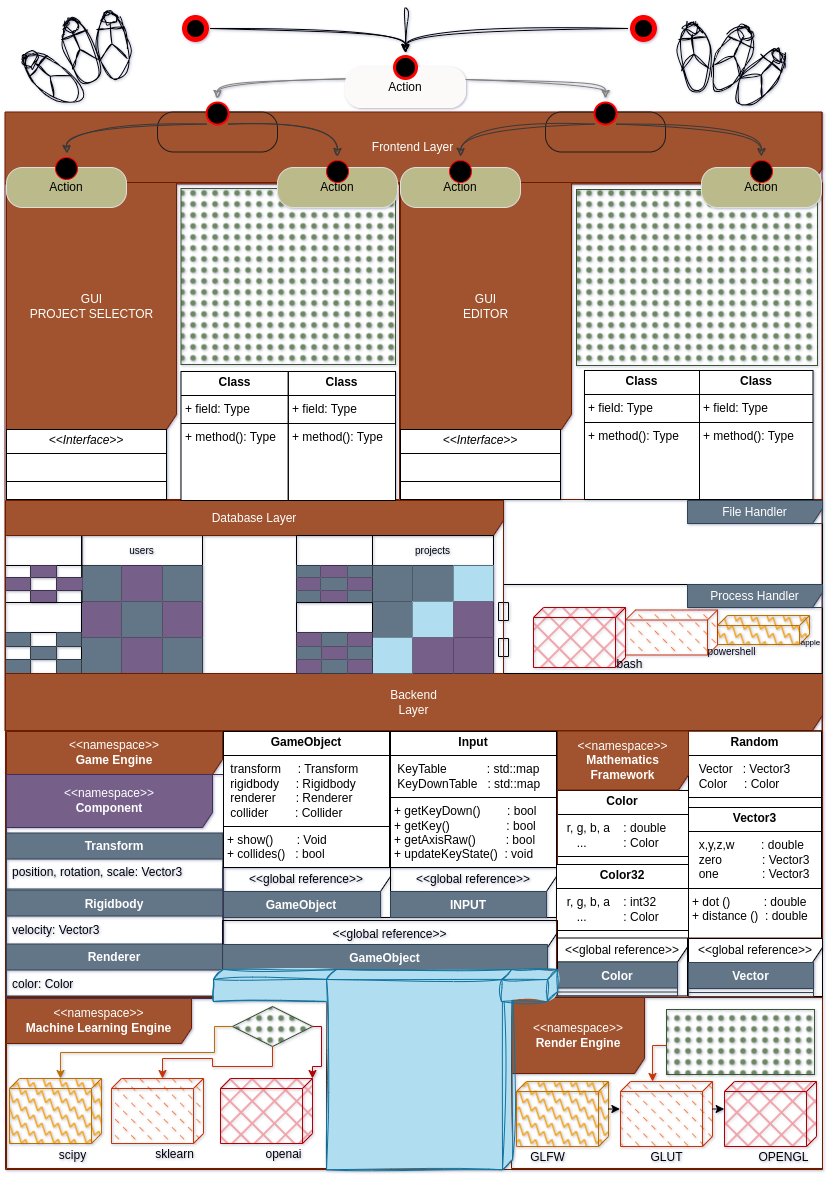
\includegraphics[width=\textwidth]{implementation_arch.png}
    \end{center}
    % \caption{}\label{fig:}
  \end{figure}
  


  % \pagebreak

  In case you haven't read the previous chapter i advise glimsing over the chapters' titles at least once because it would give better context on where my project lives in the graphics lifecycle.

  My Application is a Graphics Abstraction Layer that imitates industry standards when it comes to procedures used for ease of learning.
  Besides being an easy-to-use beginner-friendly tool because of following industry standard solution in the c++ rendering backend engine. At it's core, this rendering engine is built on top of a vectorial mathematics engine.

  The novelty that this project brings to the computer graphics world is the presence of a python Machine Learning backend that acts as an abstraction layer for simplifying the communication with services (openai, ollama) or with powerful machine learning libraries (scipy, skilearn) 


  % TODO: DIAGRAM OF python frontend AND c++/Python backend  
  

  % TODO: DRAW>IO DRAWINGS FOR ALL OF THOSE
  \section*{The C++    backend}
  % \addcontentsline{toc}{section}{Backend}
  \section*{The Python backend}

  \section*{The C++    frontend programming interface}
  % \addcontentsline{toc}{section}{Frontend}
  \section*{The Python frontend programming interface}

  \section*{interface for communicating with openai}
  % \addcontentsline{toc}{section}{openai, oLlama}
  \section*{interface for communicating with scipy}
  % \addcontentsline{toc}{section}{SciPy, SkiLearn}
  \section*{tool for web crawling}
  % \addcontentsline{toc}{section}{Data Crawling}

